
\subsection{Estudi numèric} \label{sec:estudi_numeric}

%En aquesta secció s'estudia la discretització espacial i temporal del domini. Més endavant es discretitza l'equació \eqref{eq:edp_problema} per a cada tipus de node i es proposa un algoritme de resolució.

\subsubsection{Discretització espacial} \label{sec:discretitzacio_espacial}

Existeixen dos tipus de discretitzacions espacials adequades en problemes de conducció de calor:
\begin{itemize}
	\item En la discretització per cares centrades, es col·loquen els nodes de discretització i es genera un volum de control centrat en el node. 
	\item En la discretització per nodes centrats es comença determinant els volums de control i seguidament es situa un node al centre de cadascun. En els límits del domini d'estudi també s'acostuma a col·locar nodes de discretització.
\end{itemize}

\noindent
La discretització per nodes centrats densifica la malla en les fronteres del domini d'estudi. Per aquesta raó resulta més adient pel cas actual. No obstant això, aquesta discretització genera quatre nodes singulars a les cantonades. Aquests seran tractats de forma particular posteriorment.

Donada la geometria del problema, les fronteres dels volums de control han de coincidir en la zona de contacte entre dos materials. Horitzontalment, els materials $M_1$ i $M_3$ es discretitzen en $N_1$ VC i els materials $M_2$ i $M_4$ en $N_2$ VC. Verticalment, el material $M_1$ es discretitza en $L_1$ VC i el material $M_4$ en $L_3$ VC. La zona de contacte entre $M_2$ i $M_3$ es discretitza verticalment en $L_2$ VC. Per conveniència, es defineix $N = N_1 + N_2$ i $L = L_1 + L_2 + L_3$. A la figura \ref{fig:discretització_espacial} es representa un esquema de discretització espacial.
\begin{figure}[ht]
	\centering
	\begin{tikzpicture}
		% Fill
		\fill[fill=cyan!70!white] (0,0) rectangle (5*8/11,4*8/11);
		\fill[fill=meatColor!70!white] (5*8/11,0) rectangle (11*8/11,7*8/11);
		\fill[fill=green!70!white] (0,4*8/11) rectangle (5*8/11,8*8/11);
		\fill[fill=red!70!white] (5*8/11,7*8/11) rectangle (11*8/11,8*8/11);
		% Estructura
		\draw[black, line width=0.4mm] (5*8/11,0) -- ++(0,8*8/11);
		\draw[black, line width=0.4mm] (0,4*8/11) -- ++(5*8/11,0);
		\draw[black, line width=0.4mm] (5*8/11,7*8/11) -- ++(6*8/11,0);
		\draw[black, line width=0.5mm] (0,0) -- ++(11*8/11,0) -- ++(0,8*8/11) -- ++(-11*8/11,0) -- cycle;
		% Discretizacion horizontal azul-verde
		\foreach \x in {1,2,3,4}
			\draw[black, line width=0.3mm, dashed] ({\x*8/11},0) -- ++(0,8*8/11);
		% Discretizacion horizontal rojo-carne
		\foreach \x in {1,...,7}
			\draw[black, line width=0.3mm, dashed] ({0.75*\x*8/11+5*8/11},0) -- ++(0,8*8/11);
		% Discretizacion vertical azul-carne
		\foreach \y in {1,...,4}
			\draw[black, line width=0.3mm, dashed] (0,{\y*8/11}) -- ++(11*8/11,0);
		% Discretizacion vertical verde-carne
		\foreach \y in {0,...,5}
			\draw[black, line width=0.3mm, dashed] (0,{0.5*\y*8/11+4*8/11}) -- ++(11*8/11,0);
		% Discretizacion vertical verde-rojo
		\foreach \y in {0,...,4}
			\draw[black, line width=0.3mm, dashed] (0,{0.25*\y*8/11+7*8/11}) -- ++(11*8/11,0);
		% Nodos azul		
		\foreach \x in {0,...,4}
			\foreach \y in {0,...,3}
				\filldraw[blue] ({\x*8/11+4/11},{\y*8/11+4/11}) circle (1pt);
		% Discretizacion verde 1
		\foreach \x in {0,...,4}
			\foreach \y in {0,...,5}
				\filldraw[blue] ({\x*8/11+4/11},{0.5*\y*8/11+0.25*8/11+4*8/11}) circle (1pt);
		\foreach \x in {0,...,4}
			\foreach \y in {0,...,3}
				\filldraw[blue] ({\x*8/11+4/11},{0.25*\y*8/11+0.125*8/11+7*8/11}) circle (1pt);
		% Discretizacion rojo
		\foreach \x in {0,...,7}
			\foreach \y in {0,...,3}
				\filldraw[blue] ({0.75*\x*8/11+0.375*8/11+5*8/11},{0.25*\y*8/11+0.125*8/11+7*8/11}) circle (1pt);
		% Nodos carne
		\foreach \x in {0,...,7}
			\foreach \y in {0,...,3}
				\filldraw[blue] ({0.75*\x*8/11+0.375*8/11+5*8/11},{\y*8/11+4/11}) circle (1pt);
		\foreach \x in {0,...,7}
			\foreach \y in {0,...,5}
				\filldraw[blue] ({0.75*\x*8/11+0.375*8/11+5*8/11},{0.5*\y*8/11+0.25*8/11+4*8/11}) circle (1pt); 
		% Contorno azul horizontal		
		\foreach \x in {0,...,4}
			\filldraw[blue] ({\x*8/11+4/11},0) circle (1pt);
		% Contorno carne horizontal
		\foreach \x in {0,...,7}
			\filldraw[blue] ({0.75*\x*8/11+0.375*8/11+5*8/11},0) circle (1pt);
		% Contorno verde horizontal		
		\foreach \x in {0,...,4}
			\filldraw[blue] ({\x*8/11+4/11},8*8/11) circle (1pt);
		% Contorno rojo horizontal
		\foreach \x in {0,...,7}
			\filldraw[blue] ({0.75*\x*8/11+0.375*8/11+5*8/11},8*8/11) circle (1pt);
		% Contorno azul vertical		
		\foreach \y in {0,...,3}
			\filldraw[blue] (0,{\y*8/11+4/11}) circle (1pt);
		% Contorno carne vertical 1
		\foreach \y in {0,...,3}
			\filldraw[blue] (11*8/11,{\y*8/11+4/11}) circle (1pt);
		% Contorno verde vertical 1		
		\foreach \y in {0,...,5}
			\filldraw[blue] (0,{0.5*\y*8/11+0.25*8/11+4*8/11}) circle (1pt);
		% Contorno carne vertical 2		
		\foreach \y in {0,...,5}
			\filldraw[blue] (11*8/11,{0.5*\y*8/11+0.25*8/11+4*8/11}) circle (1pt);
		% Contorno verde vertical 2
		\foreach \y in {0,...,3}
			\filldraw[blue] (0,{0.25*\y*8/11+0.125*8/11+7*8/11}) circle (1pt);
		% Contorno rojo vertical 
		\foreach \y in {0,...,3}
			\filldraw[blue] (11*8/11,{0.25*\y*8/11+0.125*8/11+7*8/11}) circle (1pt);
		% Nodos esquinas
		\filldraw[blue] (0,0) circle (1pt);
		\filldraw[blue] (11*8/11,0) circle (1pt);
		\filldraw[blue] (0,8*8/11) circle (1pt);
		\filldraw[blue] (11*8/11,8*8/11) circle (1pt);
		
		% Test
		\draw [thick, decoration={brace,raise=0cm},decorate] (0,8*8/11+0.25) -- ++(5*8/11,0)
		node [pos=0.5,anchor=north,yshift=0.7cm] {$N_1$};
		\draw [thick, decoration={brace,raise=0cm},decorate] (5*8/11,8*8/11+0.25) -- ++(6*8/11,0)
		node [pos=0.5,anchor=north,yshift=0.7cm] {$N_2$};
		\draw [thick, decoration={brace,mirror,raise=0cm},decorate] (11*8/11+0.25,0) -- ++(0,4*8/11)
		node [pos=0.5,anchor=west,xshift=0.2cm] {$L_1$};
		\draw [thick, decoration={brace,mirror,raise=0cm},decorate] (11*8/11+0.25,4*8/11) -- ++(0,3*8/11)
		node [pos=0.5,anchor=west,xshift=0.2cm] {$L_2$};
		\draw [thick, decoration={brace,mirror,raise=0cm},decorate] (11*8/11+0.25,7*8/11) -- ++(0,1*8/11)
		node [pos=0.5,anchor=west,xshift=0.2cm] {$L_3$};
		% Ejes
		\draw[<->, black, line width=0.5mm] (-0.5,1) node[above]{$j$} -- (-0.5,-0.5) -- (1,-0.5) node[right]{$i$};
	\end{tikzpicture}
	\captionsetup{width=0.45\linewidth}
	\caption{Discretització espacial.}
	\label{fig:discretització_espacial}
\end{figure}

\noindent
Un tipus de discretització amb interés és la discretització espacial uniforme. Igualant dimensions dels volums de control, s'obté una discretització uniforme si i només si es satisfan les igualtats següents
\begin{equation} \label{eq:malla_uniforme}
	\frac{1}{2 N_1} = 
	\frac{3}{5 N_2} = 
	\frac{2}{5 L_1} = 
	\frac{3}{10 L_2} = 
	\frac{1}{10 L_3},
	\quad
	N_1, N_2, L_1, L_2, L_3 \in \n
\end{equation}


\subsubsection{Discretització temporal}

\noindent
Es considera un interval de temps $[0, t_\text{max}]$. Aquest interval es discretitza en $K+1$ punts, $0 \leq t^0 < t^1 < \cdots < t^{K-1} < t^{K} \leq t_\text{max}$. A la figura \eqref{fig:discretitzacio_espacial_temporal} es mostra un esquema de la discretització temporal per a cada node.


\begin{figure}[h]
	\centering
	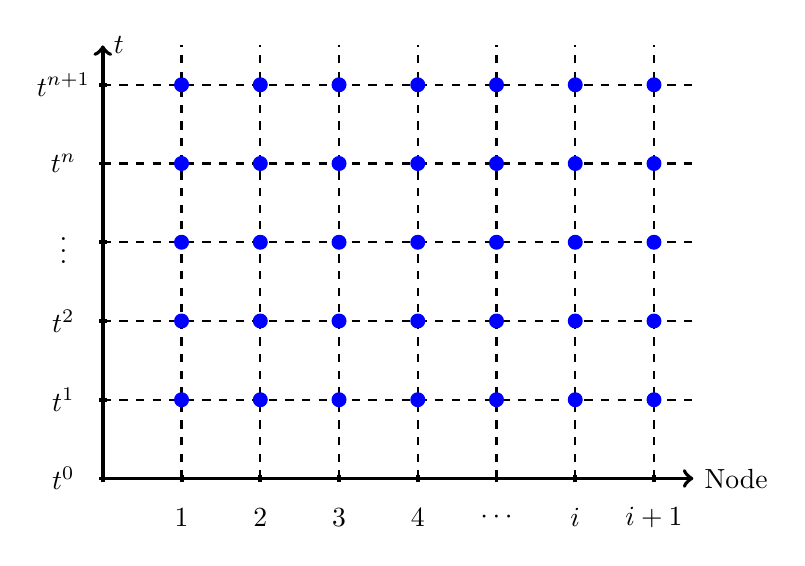
\begin{tikzpicture}
		% Ejes
		\draw[<->, line width=0.5mm] (0,5.5) node[right]{$t$}-- (0,0) -- (7.5,0) node[right]{Node};
		% Marcas tiempo
		\foreach \t in {0,...,5}
			\draw[line width=0.5mm] (-0.05,\t) -- (0.05,\t);
		\node[black] at (-0.5,0) {$t^0$};
		\node[black] at (-0.5,1) {$t^1$};
		\node[black] at (-0.5,2) {$t^2$};
		\node[black] at (-0.5,3) {$\vdots$};
		\node[black] at (-0.5,4) {$t^n$};
		\node[black] at (-0.5,5) {$t^{n+1}$};
		% Marcas nodo
		\foreach \t in {0,...,7}
			\draw[line width=0.5mm] (\t,-0.05) -- (\t,0.05);
		\node[black] at (1,-0.5) {$1$};
		\node[black] at (2,-0.5) {$2$};
		\node[black] at (3,-0.5) {$3$};
		\node[black] at (4,-0.5) {$4$};
		\node[black] at (5,-0.5) {$\cdots$};
		\node[black] at (6,-0.5) {$i$};
		\node[black] at (7,-0.5) {$i+1$};
		% Líneas horizontales
		\foreach \t in {1,...,5}
			\draw[line width=0.3mm, dashed] (0,\t) -- (7.5,\t);
		% Líneas verticales
		\foreach \t in {1,...,7}
			\draw[line width=0.3mm, dashed] (\t,0) -- (\t,5.5);
		% Puntos
		\foreach \x in {1,...,7}
			\foreach \y in {1,...,5}
				\filldraw[blue] (\x,\y) circle (2.5pt);		
	\end{tikzpicture}
	\caption{Discretització temporal.}
	\label{fig:discretitzacio_espacial_temporal}
\end{figure}

\noindent
El mapa de temperatures del domini és conegut a l'instant inicial $t^0$. La temperatura és calculada instant per instant. Com resulta intuïtiu, la temperatura a l'instant $t^{n+1}$ depèn només de les temperatures als intants $t^0, \, t^1, \, \ldots, \, t^n$. Atès que el flux de calor a la paret superior no és gran i que l'increment de temperatura de la paret dreta és lent, és suficient fer una discretització uniforme de l'interval de temps. D'aquesta manera el pas de temps és $\Delta t = t_\text{max} / K$ i es té que $t^{n+1} - t^n = \Delta t$ per $n = 0 \divisionsymbol K-1$.

Pel que fa a la integració temporal, es consideren tres esquemes numèrics. Sigui $f \colon [0, t_\text{max}] \rightarrow \real$ una funció contínua. Es vol conèixer el valor de $\int_{t^n}^{t^{n+1}} f(t) \dd{t}$. No es coneix una expressió analítica per $f$, només $f_n = f(t^n)$ i $f_{n+1} = f(t^{n+1})$, per tant s'ha d'aproximar la integral. A la figura \ref{fig:esquemes_integracio_temporal} es mostren els tres esquemes d'integració temporal rellevants per l'estudi actual.
\begin{figure}[h]
	\begin{subfigure}{.33\textwidth}
		\centering
		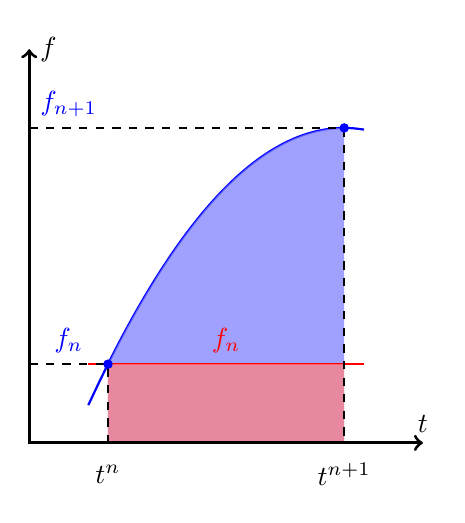
\begin{tikzpicture}			
			% Curva
			\draw[scale=1, domain=0.75:4.25, smooth, variable=\x, blue, thick] plot ({\x}, {-\x*\x/3+8*\x/3-4/3});
			\node[blue] at (0.5,1.3) {$f_n$};
			\node[blue] at (0.5,4.3) {$f_{n+1}$};
			% Shade curva
			\fill[blue!50!white, domain=1:4, variable=\x, opacity=0.75] (1, 0) -- plot ({\x}, {-\x*\x/3+8*\x/3-4/3}) -- (4,0) -- cycle;
			% Aproximacion
			\draw[scale=1, domain=0.75:4.25, smooth, variable=\x, red, thick] plot ({\x}, {1});
			\node[red] at (2.5,1.3) {$f_n$};
			% Shade aproximacion
			\fill[red!50!white, domain=1:4, variable=\x, opacity=0.75] (1, 0) -- plot ({\x}, {1}) -- (4,0) -- cycle;
			% Lineas de puntos
			\draw[line width=0.3mm, dashed] (0,1) -- (1,1) -- (1,0);
			\draw[line width=0.3mm, dashed] (0,4) -- (4,4) -- (4,0);
			% Puntos
			\filldraw[blue] (1,1) circle (1.5pt);	
			\filldraw[blue] (4,4) circle (1.5pt);
			% Ejes			
			\draw[<->, line width=0.4mm] (0,5) node[right]{$f$} -- (0,0) -- (5,0) node[above]{$t$};
			\node[black] at (1,-0.4) {$t^n$};
			\node[black] at (4,-0.4) {$t^{n+1}$};
		\end{tikzpicture}
		\caption{Explícit}
		\label{fig:esquema_explicit}
	\end{subfigure}%
	\begin{subfigure}{.33\textwidth}
		\centering
		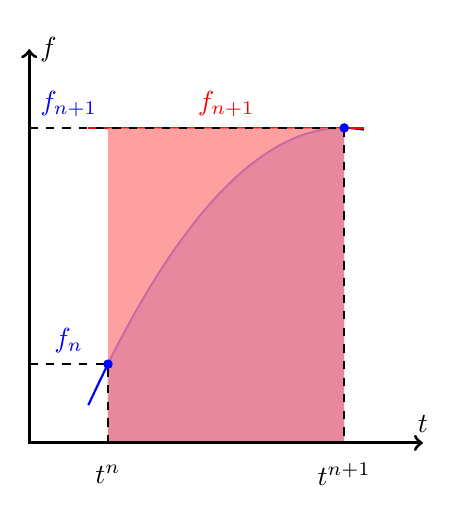
\begin{tikzpicture}
			% Curva
			\draw[scale=1, domain=0.75:4.25, smooth, variable=\x, blue, thick] plot ({\x}, {-\x*\x/3+8*\x/3-4/3});
			\node[blue] at (0.5,1.3) {$f_n$};
			\node[blue] at (0.5,4.3) {$f_{n+1}$};
			% Shade curva
			\fill[blue!50!white, domain=1:4, variable=\x, opacity=0.75] (1, 0) -- plot ({\x}, {-\x*\x/3+8*\x/3-4/3}) -- (4,0) -- cycle;
			% Aproximacion
			\draw[scale=1, domain=0.75:4.25, smooth, variable=\x, red, thick] plot ({\x}, {4});
			\node[red] at (2.5,4.3) {$f_{n+1}$};
			% Shade aproximacion
			\fill[red!50!white, domain=1:4, variable=\x, opacity=0.75] (1, 0) -- plot ({\x}, {4}) -- (4,0) -- cycle;
			% Lineas de puntos
			\draw[line width=0.3mm, dashed] (0,1) -- (1,1) -- (1,0);
			\draw[line width=0.3mm, dashed] (0,4) -- (4,4) -- (4,0);
			% Puntos
			\filldraw[blue] (1,1) circle (1.5pt);	
			\filldraw[blue] (4,4) circle (1.5pt);
			% Ejes			
			\draw[<->, line width=0.4mm] (0,5) node[right]{$f$} -- (0,0) -- (5,0) node[above]{$t$};
			\node[black] at (1,-0.4) {$t^n$};
			\node[black] at (4,-0.4) {$t^{n+1}$};
		\end{tikzpicture}
		\caption{Implícit}
		\label{fig:esquema_implicit}
	\end{subfigure}%
	\begin{subfigure}{.33\textwidth}
		\centering
		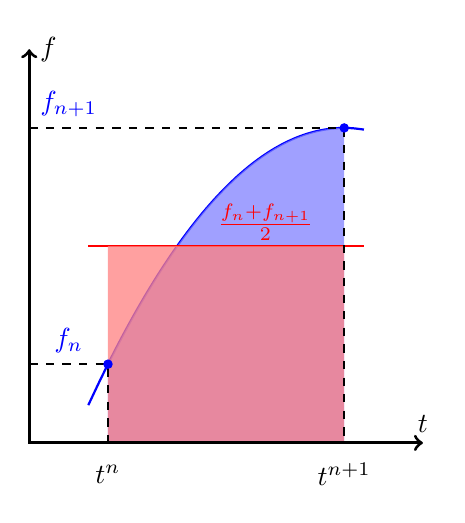
\begin{tikzpicture}
			% Curva
			\draw[scale=1, domain=0.75:4.25, smooth, variable=\x, blue, thick] plot ({\x}, {-\x*\x/3+8*\x/3-4/3});
			\node[blue] at (0.5,1.3) {$f_n$};
			\node[blue] at (0.5,4.3) {$f_{n+1}$};
			% Shade curva
			\fill[blue!50!white, domain=1:4, variable=\x, opacity=0.75] (1, 0) -- plot ({\x}, {-\x*\x/3+8*\x/3-4/3}) -- (4,0) -- cycle;
			% Aproximacion
			\draw[scale=1, domain=0.75:4.25, smooth, variable=\x, red, thick] plot ({\x}, {2.5});
			\node[red] at (3,2.8) {$\frac{f_n + f_{n+1}}{2}$};
			% Shade aproximacion
			\fill[red!50!white, domain=1:4, variable=\x, opacity=0.75] (1, 0) -- plot ({\x}, {2.5}) -- (4,0) -- cycle;
			% Lineas de puntos
			\draw[line width=0.3mm, dashed] (0,1) -- (1,1) -- (1,0);
			\draw[line width=0.3mm, dashed] (0,4) -- (4,4) -- (4,0);
			% Puntos
			\filldraw[blue] (1,1) circle (1.5pt);	
			\filldraw[blue] (4,4) circle (1.5pt);
			% Ejes			
			\draw[<->, line width=0.4mm] (0,5) node[right]{$f$} -- (0,0) -- (5,0) node[above]{$t$};
			\node[black] at (1,-0.4) {$t^n$};
			\node[black] at (4,-0.4) {$t^{n+1}$};
		\end{tikzpicture}
		\caption{Crank--Nicolson}
		\label{fig:esquema_crank-nicolson}
	\end{subfigure}
	\caption{Esquemes d'integració temporal.}
	\label{fig:esquemes_integracio_temporal}
\end{figure}

\noindent
L'estabilitat numèrica d'una solució és el comportament que presenta davant l'augment del pas de temps $\Delta t$. Si la solució es comporta bé amb passos de temps arbitràriament grans, es diu que el mètode és incondicionalment estable. Altrament, es diu que és condicionalment estable. L'esquema explícit és condicionalment estable, mentre que l'implicit i l'esquema de Crank--Nicolson són incondicionalment estables. D'altra banda, els mètodes explícit i implícit donen aproximacions de primer ordre, mentre que Crank--Nicolson dona una de segon ordre. Per més informació sobre l'ordre de l'aproximació en integració numèric, el lector por consultar a l'annex \ref{ap:calcul_numeric}.

Tal com s'aprecia a la figura \ref{fig:esquemes_integracio_temporal}, les aproximacions donades per cada esquema són, respectivament:
\begin{align}
	\int_{t^n}^{t^{n+1}} f(t) \dd{t} &\approx f_n \, \Delta t \\
	\int_{t^n}^{t^{n+1}} f(t) \dd{t} &\approx f_{n+1} \, \Delta t \\
	\int_{t^n}^{t^{n+1}} f(t) \dd{t} &\approx \frac{f_n + f_{n+1}}{2} \, \Delta t
\end{align}
De forma compacta,
\begin{equation}
	\int_{t^n}^{t^{n+1}} f(t) \dd{t} \approx \left( \beta f_{n+1} + (1 - \beta) f_n \right) \, \Delta t
\end{equation}
de manera que per $\beta = 0$ és un esquema explícit, per $\beta = 1$ un implícit i per $\beta = 1 / 2$ un esquema de Crank--Nicolson.

\subsubsection{Equació de discretització dels nodes interns \texorpdfstring{$1 \leq i \leq N, \, 1 \leq j \leq L$}{}}

En les següents seccions es desenvolupen les equacions de discretització dels diferents tipus de nodes en la discretització per nodes centrats. 

Pels nodes interns es comença plantejant el Primer Principi de la Termodinàmica en règim transitori sobre el volum de control del node $P$:
\begin{equation} \label{eq:nodes_interns_ppt}
	\pdv{t} \int_{V_P} \rho u \dd{V} = \sum \dot{Q}_P
\end{equation}
L'expressió de l'energia interna en el VC $P$ no és coneguda. Per això es defineix l'energia interna mitja del volum de control com
\begin{equation}
	\overline{u}_P = \frac{1}{\rho_P V_P} \int_{V_P} \rho u \dd{V}
\end{equation}
Atès que $\rho_P$ i $V_P$ són constants, es pot escriure \eqref{eq:nodes_interns_ppt} com:
\begin{equation} 
	\pdv{\left(\rho_P V_P \overline{u}_P\right)}{t} = 
	\rho_P V_P \pdv{\overline{u}_P}{t} =
	\sum \dot{Q}_P
\end{equation}
Integrant entre dos temps $t^n$ i $t^{n+1}$
\begin{equation} \label{eq:nodes_interns_eq_2}
	\int_{t^n}^{t^{n+1}} \rho_P V_P \pdv{\overline{u}_P}{t} \dd{t} = 
	\int_{t^n}^{t^{n+1}} \sum \dot{Q}_P \dd{t}
\end{equation}
Es desenvolupa primerament el terme esquerre de \eqref{eq:nodes_interns_eq_2}. És sabut que l'energia interna és una funció de punt, per tant la integral de $\partial \overline{u}_P / \partial t$ entre els instants $t^n$ i $t^{n+1}$ no depèn del procès seguit sino dels estats inicial i final. És raonable aproximar el sòlid per un sòlid semiperfecte i fer $\overline{u}_P \approx u_P$. La variació d'energia interna és $\dd{u} = c_p \dd{T}$. D'aquesta manera, el terme esquerre de \eqref{eq:nodes_interns_eq_2} queda
\begin{align}
	\int_{t^n}^{t^{n+1}} \rho_P V_P \pdv{\overline{u}_P}{t} \dd{t} 			&= 
	\rho_P V_P  \int_{t^n}^{t^{n+1}} \pdv{\overline{u}_P}{t} \dd{t} = 
	\rho_P V_P \left( \overline{u}_P^{n+1} - \overline{u}_P^n \right) \nonumber  \\ 	&\approx 
	\rho_P V_P \left( u_P^{n+1} - u_P^n \right) = 
	\rho_P V_P \overline{c}_{p_P} \left( T_P^{n+1} - T_P^n \right) \label{eq:nodes_interns_terme_esquerre}
\end{align}
on $\overline{c}_{p_P}$ és el calor específic mig, definit com
\begin{equation}
	\overline{c}_{p_P} = 
	\frac{1}{T_P^{n+1} - T_P^n} \int_{T_P^n}^{T_P^{n+1}} c_{p_P}(T) \dd{T} \approx c_{p_P}
\end{equation}
El terme dret de \eqref{eq:nodes_interns_eq_2} desenvolupat queda
\begin{equation} \label{eq:nodes_interns_terme_dret}
	\int_{t^n}^{t^{n+1}} \sum \dot{Q}_P \dd{t} = 
	\left( \beta \sum \dot{Q}_P^{n+1} + (1 - \beta) \sum \dot{Q}_P^n \right) \Delta t
\end{equation}
amb $\beta \in [0,1]$, que depèn de l'esquema d'integració. Introduint \eqref{eq:nodes_interns_terme_esquerre} i \eqref{eq:nodes_interns_terme_dret} en \eqref{eq:nodes_interns_eq_2} s'obté la següent expressió:
\begin{equation} \label{eq:nodes_interns_eq_3}
	\rho_P V_P c_{p_P} \frac{T_P^{n+1} - T_P^n}{\Delta t} = 
	\beta \sum \dot{Q}_P^{n+1} + (1 - \beta) \sum \dot{Q}_P^n	
\end{equation}
A la figura \ref{fig:fluxos_calor_nodes_interns} es representen els fluxos de calor en el volum de control del node $P$.
\begin{figure}[ht]
	\centering
	\begin{tikzpicture}
		% Control volumes
		\draw[black, dashed, line width=0.3mm] (-0.5,2) -- ++(7,0);
		\draw[black, dashed, line width=0.3mm] (-0.5,4) -- ++(7,0);
		\draw[black, dashed, line width=0.3mm] (2,-0.5) -- ++(0,7);
		\draw[black, dashed, line width=0.3mm] (4,-0.5) -- ++(0,7);
		\foreach \x in {0,1}			
		\draw[black, dashed, line width=0.3mm] (1.5,{6*\x}) -- ++(3,0);
		\foreach \x in {0,1}			
		\draw[black, dashed, line width=0.3mm] ({6*\x},1.5) -- ++(0,3);
		% Nodos
		\foreach \x in {0,1,2}
		\filldraw[nodeColor] ({2*\x+1},3) circle (3pt);
		\foreach \x in {0,1}
		\filldraw[nodeColor] (3,{4*\x+1}) circle (3pt);
		\node[nodeColor] at (1,3.3) {$W$};
		\node[nodeColor] at (5,3.3) {$E$};
		\node[nodeColor] at (3.3,1) {$S$};
		\node[nodeColor] at (3.3,5) {$N$};
		\node[nodeColor] at (3.3,3.3) {$P$};
		% Flujos de calor
		\draw[->,red,line width=0.3mm] (1.5,3) node[above,xshift=1mm]{$\dot{Q}_w$} -- ++(1,0);
		\draw[->,red,line width=0.3mm] (3.5,3) -- ++(1,0) node[above,xshift=-1mm]{$\dot{Q}_e$};
		\draw[->,red,line width=0.3mm] (3,1.5) node[right,yshift=1mm]{$\dot{Q}_s$} -- ++(0,1);
		\draw[->,red,line width=0.3mm] (3,3.5) -- ++(0,1) node[right,yshift=-1mm]{$\dot{Q}_n$};
		% Cotas
		\draw[<->, blue, line width=0.3mm] (2,6.25) -- node[midway, above]{$\Delta x_P$}++(2,0);
		\draw[<->, blue, line width=0.3mm] (6.25,2) -- node[midway, right]{$\Delta y_P$}++(0,2);
	\end{tikzpicture}
	\caption{Fluxos de calor en els nodes interns.}
	\label{fig:fluxos_calor_nodes_interns}
\end{figure}

\noindent
El flux de calor net sobre el volum de control del node $P$ en un instant general $t^{n}$ és
\begin{align}
	\sum \dot{Q}_P^n 
	&= 
	\dot{Q}_w^n - \dot{Q}_e^n + \dot{Q}_s^n - \dot{Q}_n^n \nonumber \\
	&\approx 
	- \lambda_w \frac{T_P^n - T_W^n}{d_{PW}} S_w 
	+ \lambda_e \frac{T_E^n - T_P^n}{d_{PE}} S_e
	- \lambda_s \frac{T_P^n - T_S^n}{d_{PS}} S_s 
	+ \lambda_n \frac{T_N^n - T_P^n}{d_{PN}} S_n \nonumber \\
	&=
	\frac{\lambda_w S_w}{d_{PW}} T_W^n + 
	\frac{\lambda_e S_e}{d_{PE}} T_E^n + 
	\frac{\lambda_s S_s}{d_{PS}} T_S^n + 
	\frac{\lambda_n S_n}{d_{PN}} T_N^n -
	\left(
	\frac{\lambda_w S_w}{d_{PW}} + 
	\frac{\lambda_e S_e}{d_{PE}} + 
	\frac{\lambda_s S_s}{d_{PS}} + 
	\frac{\lambda_n S_n}{d_{PN}}
	\right) T_P^n \label{eq:nodes_interns_fluxe_calor}
\end{align}
on s'han aproximat les derivades parcials per diferències finites centrades a les cares. Aquestes són aproximacions de segon ordre. Per més informació sobre altres aproximacions de les derivades, el lector interessat pot consultar l'annex \ref{ap:calcul_numeric}. Les conductivitats tèrmiques a les cares es calculen amb la mitja harmònica, és a dir,
\begin{align}
	\lambda_w &= \frac{d_{PW}}{d_{Pw} / \lambda_P + d_{Ww} / \lambda_W} \\
	\lambda_e &= \frac{d_{PE}}{d_{Pe} / \lambda_P + d_{Ee} / \lambda_E} \\
	\lambda_s &= \frac{d_{PS}}{d_{Ps} / \lambda_P + d_{Ss} / \lambda_S} \\
	\lambda_n &= \frac{d_{PN}}{d_{Pn} / \lambda_P + d_{Nn} / \lambda_N}
\end{align}
Les superfícies de transferència de calor són:
\begin{align}
	S_w &= S_e = W \Delta y_P \\
	S_s &= S_n = W \Delta x_P 
\end{align}
Introduint \eqref{eq:nodes_interns_fluxe_calor} en \eqref{eq:nodes_interns_eq_3} i desenvolupant s'arriba a l'equació de discretització dels nodes interns:
\begin{multline} \label{eq:equacio_discretitzacio_nodes_interns}
	\left[
		\frac{\rho_P V_P c_{p_P}}{\Delta t} + 
		\beta \left(
		\frac{\lambda_w S_w}{d_{PW}} + 
		\frac{\lambda_e S_e}{d_{PE}} + 
		\frac{\lambda_s S_s}{d_{PS}} + 
		\frac{\lambda_n S_n}{d_{PN}}
		\right)
	\right] T_P^{n+1} = \\
	=
	\beta \frac{\lambda_w S_w}{d_{PW}} T_W^{n+1} + 
	\beta \frac{\lambda_e S_e}{d_{PE}} T_E^{n+1} + 
	\beta \frac{\lambda_s S_s}{d_{PS}} T_S^{n+1} + 
	\beta \frac{\lambda_n S_n}{d_{PN}} T_N^{n+1} + 
	\frac{\rho_P V_P c_{p_P}}{\Delta t} T_P^n + 
	(1 - \beta) \sum \dot{Q}_P^n	
\end{multline}
Es defineixen els següents coeficients de discretització:
\begin{align}
	a_W &= \beta \frac{\lambda_w S_w}{d_{PW}} \\
	a_E &= \beta \frac{\lambda_e S_e}{d_{PE}} \\
	a_S &= \beta \frac{\lambda_s S_s}{d_{PS}} \\
	a_N &= \beta \frac{\lambda_n S_n}{d_{PN}} \\
	a_P &= \frac{\rho_P V_P c_{p_P}}{\Delta t} + a_W + a_E + a_S + a_N \\
	b_P &= \frac{\rho_P V_P c_{p_P}}{\Delta t} T_P^n + (1 - \beta) \sum \dot{Q}_P^n	
\end{align}
L'equació de discretització compacta pels nodes interns queda:
\begin{equation} \label{eq:equacio_discretitzacio_general}
	a_P T_P^{n+1} = 
	a_W T_W^{n+1} + 
	a_E T_E^{n+1} + 
	a_S T_S^{n+1} + 
	a_N T_N^{n+1} + 
	b_P, 
	\quad
	0 \leq n \leq n_\text{max}-1
\end{equation}

\subsubsection{Equació de discretització dels nodes inferiors \texorpdfstring{$\left( 1 \leq i \leq N, \, j = 0 \right)$}{}}

En el costat inferior es té la condició d'isoterma a $T_\text{inf} = 23 \ \celsius$, de tal manera que el node $P$ no transfereix calor amb els nodes veïns. A la figura \ref{fig:fluxos_calor_nodes_inferiors} es mostren els nodes veïns i la condició de contorn. Per tant $T_P^n = T_\text{inf}$ per a tot instant de temps $n$. Els coeficients de discretització són
\begin{align}
	a_W = a_E &= a_S = a_N = 0 \\
	a_P &= 1 \\
	b_P &= T_\text{inf}
\end{align}
L'equació de discretització compacta pels nodes inferiors és igual a l'equació \eqref{eq:equacio_discretitzacio_general}.
%\begin{equation}
%	a_P T_P^{n+1} = 
%	a_W T_W^{n+1} + 
%	a_E T_E^{n+1} + 
%	a_S T_S^{n+1} + 
%	a_N T_N^{n+1} + 
%	b_P, 
%	\quad
%	0 \leq n \leq n_\text{max}-1
%\end{equation}

\begin{figure}[ht]
	\centering
	\begin{tikzpicture}
		% VC
		\draw[black, line width=0.5mm] (-0.5,0) -- ++(7,0);
		\draw[black, dashed, line width=0.3mm] (-0.5,2) -- ++(7,0);
		\foreach \x in {0,...,3}
		\draw[black, dashed, line width=0.3mm] ({2*\x},0) -- ++(0,2.5);
		% Nodos
		\foreach \x in {0,1,2}
		\foreach \y in {0,1}
		\filldraw[nodeColor] ({2*\x+1},{\y}) circle (3pt);
		% Texto nodos
		\node[nodeColor] at (1,-0.3) {$W$};
		\node[nodeColor] at (3,-0.3) {$P$};
		\node[nodeColor] at (5,-0.3) {$E$};
		\node[nodeColor] at (3,1.3) {$N$};
		% Texto temperatura
		\node[red] at (3.5,0.3) {$T_\text{inf}$};
	\end{tikzpicture}
	\captionsetup{width=0.45\textwidth}
	\caption{Fluxos de calor en els nodes inferiors i condició de contorn.}
	\label{fig:fluxos_calor_nodes_inferiors}
\end{figure}


\subsubsection{Equació de discretització dels nodes superiors \texorpdfstring{$\left( 1 \leq i \leq N, \, j = L+1 \right)$}{}}

A la paret superior es té un flux de calor $\dot{Q}_\text{flow} = 60 \ \watt / \meter$ en direcció $y$ negativa. La longitud és per unitat de profunditat de la barra. Així el flux de calor per unitat de superfície és $\dot{q}_\text{flow} = \dot{Q}_\text{flow} / W$. Atès que no hi ha superfície de transferència de calor entre els nodes $W$, $P$ i $E$, no hi ha flux de calor entre aquests. En la figura \ref{fig:fluxos_calor_nodes_superiors} es mostren els fluxos de calor i la condició de contorn. 

\begin{figure}[ht]
	\centering
	\begin{tikzpicture}
		% VC
		\draw[black, line width=0.5mm] (-0.5,0) -- ++(7,0);
		\draw[black, dashed, line width=0.3mm] (-0.5,-2) -- ++(7,0);
		\foreach \x in {0,...,3}
			\draw[black, dashed, line width=0.3mm] ({2*\x},0) -- ++(0,-2.5);
		% Texto nodos
		\node[nodeColor] at (2.7,0.3) {$P$};
		\node[nodeColor] at (3,-1.3) {$S$};
		\node[nodeColor] at (1,0.3) {$W$};
		\node[nodeColor] at (5,0.3) {$E$};
		% Flujos de calor
		\draw[<-,red,line width=0.3mm] (3,-0.1) -- node[midway, right]{$\dot{Q}_s$} ++(0,-0.8);
		\draw[<-,red,line width=0.3mm] (3,0.1) -- node[midway, right]{$\dot{Q}_\text{sup}$} ++(0,0.8);
		% Nodos
		\foreach \x in {0,1,2}
			\foreach \y in {0,1}
				\filldraw[nodeColor] ({2*\x+1},{-\y}) circle (3pt);
		% Cota
		\draw[<->, blue, line width=0.3mm] (2,-3) -- node[midway,above]{$\Delta x_P$}++(2,0);
		\draw[blue, line width=0.3mm] (2,-2.5) -- ++(0,-0.6);
		\draw[blue, line width=0.3mm] (4,-2.5) -- ++(0,-0.6);
	\end{tikzpicture}
	\captionsetup{width=0.45\textwidth}
	\caption{Fluxos de calor en els nodes superiors i condició de contorn.}
	\label{fig:fluxos_calor_nodes_superiors}
\end{figure}

\noindent
Es parteix de l'equació \eqref{eq:nodes_interns_ppt}. Donat que $V_P = 0$, el terme esquerre és zero, de manera que la calor neta en tot instant de temps és nul·la, \ie,
\begin{equation} \label{eq:nodes_superiors_01}
	\sum \dot{Q}_P^n = 
	\dot{Q}_\text{sup}^n + \dot{Q}_s^n = 
	\dot{q}_\text{flow} W \Delta x_P - 
	\lambda_s \frac{T_P^n - T_S^n}{d_{PS}} S_s = 0
\end{equation}
on la conductivitat tèrmica i la superfície són
\begin{align}
	\lambda_s &= \frac{d_{PS}}{d_{Ps}/\lambda_P + d_{Ss}/\lambda_S} = \lambda_S \\
	S_s &= W \Delta x_p 
\end{align}
Simplificant i reordenant \eqref{eq:nodes_superiors_01} per l'instant $t^{n+1}$ s'obté
\begin{equation} \label{eq:equacio_discretitzacio_nodes_superiors}
	\frac{\lambda_s}{d_{PS}} T_P^{n+1} = 
	\frac{\lambda_s}{d_{PS}} T_S^{n+1} + 
	\dot{q}_\text{flow}
\end{equation}
Els coeficients de discretització pels nodes superiors són els següents:
\begin{align}
	a_W &= a_E = a_N = 0 \\
	a_S &= \frac{\lambda_s}{d_{PS}} \\
	a_P &= a_S \\
	b_P &= \dot{q}_\text{flow}
\end{align}
%L'equació de discretització dels nodes interns queda:
%\begin{equation}
%	a_P T_P^{n+1} = 
%	a_W T_W^{n+1} + 
%	a_E T_E^{n+1} + 
%	a_S T_S^{n+1} + 
%	a_N T_N^{n+1} + 
%	b_P, \quad 
%	0 \leq n \leq n_\text{max} - 1
%\end{equation}

\subsubsection{Equació de discretització dels nodes esquerres \texorpdfstring{$\left( i = 0, \, 1 \leq j \leq L \right)$}{}}

A la paret esquerre es té un fluid a $T_g = 33 \ \celsius$ amb un coeficient de transferència de calor $\alpha = 9 \ \watt / \meter^2 \kelvin$. Com $V_P = 0$, el terme esquerre de \eqref{eq:nodes_interns_ppt} s'anul·la. Així, la calor neta en qualsevol instant de temps és zero. A la figura \ref{fig:fluxos_calor_nodes_esquerres} es representen els fluxos de calor sobre el node $P$:
\begin{figure}[ht]
	\centering
	\begin{tikzpicture}
		% VC
		\draw[black, line width=0.5mm] (0,-0.5) -- ++(0,7);
		\draw[black, dashed, line width=0.3mm] (2,-0.5) -- ++(0,7);
		\foreach \y in {0,...,3}t
			\draw[black, dashed, line width=0.3mm] (0,{2*\y}) -- ++(2.5,0);
		% Nodos
		\foreach \x in {0,1,2}
			\foreach \y in {0,1}
				\filldraw[nodeColor] ({\y},{2*\x+1}) circle (3pt);
		% Texto nodos
		\node[nodeColor] at (-0.3,2.7) {$P$};
		\node[nodeColor] at (-0.3,5) {$N$};
		\node[nodeColor] at (-0.3,1) {$S$};
		\node[nodeColor] at (1.0,3.3) {$E$};
		% Flujos de calor
		\draw[->,red,line width=0.3mm] (0.1,3) -- node[midway, above]{$\dot{Q}_e$} ++(0.8,0);
		\draw[<-,red,line width=0.3mm] (-0.1,3) -- node[midway, above]{$\dot{Q}_\text{conv}$} ++(-0.8,0);				
		% Fluido
		\node[red] at (-2, 3) {\begin{tabular}{c} $\alpha_g$ \\ $T_g$ \end{tabular}};
		% Cota
		\draw[<->, blue, line width=0.3mm] (2.25,2) -- node[midway, right]{$\Delta y_P$}++(0,2);
		
		
		\draw[thick, red, -latex] ({0.8*cos(-120)-2},{2*sin(-120)+3}) arc (-120:120:0.8cm and 2cm);
	\end{tikzpicture}
	\caption{Fluxos de calor en els nodes esquerres.}
	\label{fig:fluxos_calor_nodes_esquerres}
\end{figure}

\noindent
En un instant qualsevol $t^n$, el flux de calor net sobre $P$ és:
\begin{equation} \label{eq:nodes_esquerres_01}
	\sum \dot{Q}_P^n = 
	\dot{Q}_\text{conv}^n - \dot{Q}_e^n =
	\alpha_g \left( T_g - T_P^n \right) S_\text{conv} + 
	\lambda_e \frac{T_E^n - T_P^n}{d_{PE}} S_e = 0
\end{equation}
on la conductivitat tèrmica i les superfícies són
\begin{align}
	\lambda_e &= \frac{d_{PE}}{d_{Pe}/\lambda_P + d_{Ee}/\lambda_E} = \lambda_E \\
	S_e &= S_\text{conv} = W \Delta y_P 
\end{align}
Simplificant \eqref{eq:nodes_esquerres_01} i reordenant termes s'arriba 
\begin{equation} \label{eq:equacio_discretitzacio_nodes_esquerres}
	\left( \frac{\lambda_e}{d_{PE}} + \alpha_g \right) T_P^{n+1} = 
	\frac{\lambda_e}{d_{PE}} T_E^{n+1} + \alpha_g T_g
\end{equation}
Els coeficients de discretització pels nodes esquerres són
\begin{align}
	a_W &= a_S = a_N = 0 \\
	a_E &= \frac{\lambda_e}{d_{PE}} \\
	a_P &= a_E + \alpha_g \\
	b_P &= \alpha_g T_g
\end{align}
%D'aquesta forma, l'equació de discretització dels nodes esquerres és:
%\begin{equation}
%	a_P T_P^{n+1} = 
%	a_W T_W^{n+1} + 
%	a_E T_E^{n+1} + 
%	a_S T_S^{n+1} + 
%	a_N T_N^{n+1} + b_P,
%	\quad
%	0 \leq n \leq n_\text{max}-1
%\end{equation}


\subsubsection{Equació de discretització dels nodes drets \texorpdfstring{$\left( i = N+1, \, 1 \leq j \leq L \right)$}{}}

Sobre la paret dreta la temperatura és $T_d(t) = 8.00 + 0.005 t \ \celsius$, on $t$ és el temps en segons. Com s'aprecia a la figura \ref{fig:fluxos_calor_nodes_drets}, no hi ha flux de calor sobre el node $P$.

\begin{figure}[ht]
	\centering
	\begin{tikzpicture}
		% VC
		\draw[black, line width=0.5mm] (2,-0.5) -- ++(0,7);
		\draw[black, dashed, line width=0.3mm] (0,-0.5) -- ++(0,7);
		\foreach \y in {0,...,3}
			\draw[black, dashed, line width=0.3mm] (2,{2*\y}) -- ++(-2.5,0);
		% Nodos
		\foreach \x in {0,1,2}
			\foreach \y in {0,1}
				\filldraw[nodeColor] ({1+\y},{2*\x+1}) circle (3pt);
		% Texto nodos
		\node[nodeColor] at (2.3,3.3) {$P$};
		\node[nodeColor] at (1.0,3.3) {$W$};
		\node[nodeColor] at (2.3,1) {$S$};
		\node[nodeColor] at (2.3,5) {$N$};		
		% Temperatura
		\node[red, anchor=west] at (2,4) {$T_d(t)$};
	\end{tikzpicture}
	\captionsetup{width=0.45\textwidth}
	\caption{Fluxos de calor en els nodes drets i condició de contorn.}
	\label{fig:fluxos_calor_nodes_drets}
\end{figure}

\noindent
La temperatura del node $P$ en l'instant $t^{n+1}$ és
\begin{equation}
	T_P^{n+1} = 8.00 + 0.005 t^{n+1}
\end{equation}
Els coeficients de discretització per aquest tipus de node són:
\begin{align}
	a_W &= a_E = a_S = a_N = 0 \\
	a_P &= 1 \\
	b_P &= 8.00 + 0.005 t^{n+1}
\end{align}


\subsubsection{Nodes singulars}

En l'anàlisi anterior no han aparegut els nodes de les cantonades, \ie, els nodes $[1][1]$, $[N+2][1]$, $[1][L+2]$ i $[N+2][L+2]$. Això indica aquests nodes i els nodes veïns no s'influeixen, motiu pel qual reben el nom de nodes singulars. La temperatura dels nodes singulars pot ser assignada de manera arbitrària. Tanmateix, si es desitja representar una superfície de temperatura $T(t^n, x, y)$ o es volen trobar les corbes isotermes, és necessari la temperatura dels nodes estigui relacionada amb el seu entorn.

Atès que els nodes $[1][1]$ i $[N+2][1]$ pertanyen a la paret inferior, s'imposa que la seva temperatura sigui la d'isoterma a $T_\text{inf} = 23 \ \celsius$ per a tot instant de temps.

En el node $[1][L+2]$ es fa que la temperatura sigui la mitja aritmètica de les temperatures dels nodes veïns $S$ i $E$, és a dir,
\begin{equation}
	T_P = T[1][L+2] = \frac{T[1][L+1] + T[2][L+2]}{2} = \frac{T_S + T_E}{2}
\end{equation} 

Per últim, el node $[N+2][L+2]$ es troba a la pared dreta, on hi ha condició de temperatura creixent, de manera que s'imposa que la seva temperatura sigui igual a la de paret. 

\subsubsection{Algoritme de resolució}

A continuació es mostra l'algoritme de resolució proposat per \cite{cttc}.
\begin{algorithm}[h]
	\caption{Algoritme de resolució 1}
	\label{algorithm:algoritme_resolucio_1}
	\begin{algorithmic}[0]
		\State 
		\begin{enumerate}[label=\textbf{\arabic*}]
			\item Entrada de dades:
			\begin{enumerate}[label=\textbf{1.\arabic*}]
				\item Dades físiques: geometria, propietats termofísiques dels materials, condicions de contorn, condicions inicials.
				\item Dades numèriques: malla, $\Delta t$ (increment de temps), $\delta$ (criteri de convergència), $\beta$.
			\end{enumerate}
			\item Càlculs previs: generació de la malla, distàncies, superfícies, volums.
			\item Mapa inicial de temperatures $(t^n = 0)$: $n \gets 0$, $T^n[i][j] = T_0(x,y)$.
			\item Càlcul del següent instant de temps: $t^{n+1} = t^n + \Delta t$. Estimació del mapa de temperatures $T^{n+1 \, \ast}[i][j] = T^n[i][j]$. \label{enum:algoritme_4}
			\item Avaluació dels coeficients de discretització: $a_W, \, a_E, \, a_S, \, a_N, \, a_P, \, b_P$ a cada node $[i][j]$. \label{enum:algoritme_5}
			\item Resolució del sistema d'equacions \label{enum:algoritme_6}
			\vspace*{-3mm}
			\begin{multline*}
				a_P[i][j] \, T^{n+1}[i][j] =  
				a_W[i][j] \, T^{n+1}[i-1][j] + 
				a_E[i][j] \, T^{n+1}[i+1][j] + \\ +
				a_S[i][j] \, T^{n+1}[i][j-1] + 
				a_N[i][j] \, T^{n+1}[i][j+1] + 
				b_P[i][j]
			\end{multline*}
			\item És $\max{\abs{T^{n+1 \, \ast}[i][j] - T^{n+1}[i][j]}} < \delta$? \label{enum:algoritme_7}
			\begin{itemize}
				\item Sí: continua.
				\item No: $T^{n+1 \, \ast}[i][j] \gets T^{n+1}[i][j]$, torna a \ref{enum:algoritme_5}
			\end{itemize}
			\item Nou instant de temps?
			\begin{itemize}
				\item Sí: $n \gets n + 1$, torna a \ref{enum:algoritme_4}
				\item No: continua.
			\end{itemize}
			\item Càlculs finals i impressió de resultats.
			\item Fi.
		\end{enumerate}
	\end{algorithmic}
\end{algorithm}

Aquest algoritme és un algoritme general per conducció bidimensional, adequat en casos on les propietats termofísiques ($\rho$, $c_p$ i $\lambda$) depenen de la temperatura. Com aquestes propietats apareixen en els coeficients de discretització, si la condició de convergència del pas \ref{enum:algoritme_7} no es satisfà, és necessari recalcular els coeficients amb les propietats termofísiques a la nova temperatura $T^{n+1}[i][j]$.

Com s'ha vist, els coeficients de discretització no depenen en cap cas de la de temperatura en l'instant $t^{n+1}$. Els coeficients $a_W, \, a_E, \, a_S, \, a_N, \, a_P$ de qualsevol node depenen, en general, de l'esquema d'integració, de la conductivitat tèrmica a la cara corresponent i de la geometria. Donat que les propietats termofísiques són constants i la geometria del problema és invariant, els coeficients esmentats són constants al llarg de l'execució de l'algoritme. En conseqüència, només és necessari calcular-los una vegada.

Pels nodes de les parets inferior, superior i esquerre, el coeficient de discretització $b_P$ és també constant. L'assignació en memòria d'aquests coeficients es pot fer des d'un principi, en lloc d'iteració per iteració. 

A l'algoritme \ref{algorithm:algoritme_resolucio_2} es mostra la millora. Cal notar que aquest és un cas particular de l'algoritme \ref{algorithm:algoritme_resolucio_1}, per tant es redueix el seu rang d'aplicació. No obstant això, redueix el nombre d'operacions necessàries, millorant el temps d'execució.

\begin{algorithm}[h]
	\caption{Algoritme de resolució 2}
	\label{algorithm:algoritme_resolucio_2}
	\begin{algorithmic}[0]
		\State 
		\begin{enumerate}[label=\textbf{\arabic*}]
			\item Entrada de dades:
			\begin{enumerate}[label=\textbf{1.\arabic*}]
				\item Dades físiques: geometria, propietats termofísiques dels materials, condicions de contorn, condicions inicials.
				\item Dades numèriques: malla, $\Delta t$ (increment de temps), $\delta$ (criteri de convergència), $\beta$.
			\end{enumerate}
			\item Càlculs previs: generació de la malla, distàncies, superfícies, volums i conductivitats tèrmiques a les cares. Avaluació dels coeficients de discretització $a_W, \, a_E, \, a_S, \, a_N, \, a_P$ i dels coeficients $b_P$ constants.
			\item Mapa inicial de temperatures $(t^n = 0)$: $n \gets 0$, $T^n[i][j] = T_0(x,y)$.
			\item Càlcul del següent instant de temps: $t^{n+1} = t^n + \Delta t$. Estimació del mapa de temperatures $T^{n+1 \, \ast}[i][j] \gets T^n[i][j]$. \label{enum:algoritme2_4}
			\item Avaluació dels coeficients de discretització variables $b_P$ a cada node $[i][j]$. \label{enum:algoritme2_5}
			\item Resolució del sistema d'equacions \label{enum:algoritme2_6}
			\vspace*{-3mm}
			\begin{multline*}
				a_P[i][j] \, T^{n+1}[i][j] =  
				a_W[i][j] \, T^{n+1}[i-1][j] + 
				a_E[i][j] \, T^{n+1}[i+1][j] + \\ +
				a_S[i][j] \, T^{n+1}[i][j-1] + 
				a_N[i][j] \, T^{n+1}[i][j+1] + 
				b_P[i][j]
			\end{multline*}
			\item És $\max{\abs{T^{n+1 \, \ast}[i][j] - T^{n+1}[i][j]}} < \delta$? \label{enum:algoritme2_7}
			\begin{itemize}
				\item Sí: continua.
				\item No: $T^{n+1 \, \ast}[i][j] \gets T^{n+1}[i][j]$, torna a \ref{enum:algoritme2_6}
			\end{itemize}
			\item Nou instant de temps?
			\begin{itemize}
				\item Sí: $n \gets n + 1$, torna a \ref{enum:algoritme2_4}
				\item No: continua.
			\end{itemize}
			\item Càlculs finals i impressió de resultats.
			\item Fi.
		\end{enumerate}
	\end{algorithmic}
\end{algorithm}

Com es pot comprovar fàcilment, si s'ordena el sistema d'equacions de manera adequada, s'obté una matriu pentadiagonal. Si el nombre de nodes de discretitació és gran, s'obté una matriu dispersa, \ie, una matriu on la majoria d'entrades són zero. Això fa que no sigui adequat guardar els coeficients $a_i$ en una matriu quadrada. 

La resolució del sistema d'equacions es fa per un mètode \emph{point--by--point}. Els passos \ref{enum:algoritme2_6} i \ref{enum:algoritme2_7} de l'algoritme \ref{algorithm:algoritme_resolucio_2} són l'algoritme de Gauss--Seidel. El lector interessat pot trobar un altre mètode de resolució de sistemes lineals, la factorització $L U$, en l'annex \ref{ap:sistemes_lineals}. Ara bé, donada la natura de la matriu de coeficients del sistema, aquest mètode no és adequat si el nombre de nodes de discretització és gran. 

A partir de les equacions dels nodes de discretització, es pot comprovar que aquets satisfan la condició de matriu diagonalment dominant per files
\begin{equation}
	\abs{a_P} \geq \abs{a_W} + \abs{a_E} + \abs{a_S} + \abs{a_N}
\end{equation}
Això assegura que el mètode de Gauss-Seidel convergeix.



